\documentclass[9pt, aspectratio=169]{beamer}
\usepackage{FiraSans}
\usetheme[subsectionpage=progressbar]{metropolis}
\usepackage[utf8]{inputenc}
\usepackage{amsmath}
\usepackage{amsfonts}
\usepackage{amssymb}
\usepackage{multicol}
\usepackage{tikz}
\usetikzlibrary{matrix}
\usepackage{caption}
\usepackage{xcolor}
\usepackage[T1]{fontenc} 
\usepackage[skins]{tcolorbox}
\author{Nicola Roman\`o - nicola.romano@ed.ac.uk}
\title{Lecture 17 - Hyperparameter tuning}
\setlength{\fboxsep}{0pt}
\setbeamertemplate {footline}{\begin{scriptsize}\hfill\insertframenumber ~of \inserttotalframenumber\kern1em\vskip5pt\end{scriptsize}}

% Remove "Figure" in front of captions
% See https://tex.stackexchange.com/questions/82456/how-to-remove-figure-caption-prefix-figure-in-beamer
\captionsetup{labelformat=empty,labelsep=none}

\titlegraphic{\centering 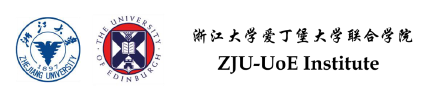
\includegraphics[scale=.5]{instituteLogo.png}}
\date{}

\begin{document}

\newtcolorbox{codebox}{enhanced,
    top=2pt,
    left=2pt,
    right=2pt,
    bottom=2pt,
    boxrule=0pt,
    leftrule=5pt,
    sharp corners,
    colback=gray!20,
    colframe=blue!60!black}

\begin{frame}
    \titlepage
\end{frame}

\begin{frame}
    {Learning objectives}
    \begin{columns}
        \begin{column}{0.8\textwidth}
            \begin{itemize}
                \item Give examples of hyperparameters and explain what are the issues with hyperparameters in deep learning.
                \item Discuss and compare different methods of tuning hyperparameters.
                \item Implement these methods in Python.
            \end{itemize}
        \end{column}
        \begin{column}{0.2\textwidth}
            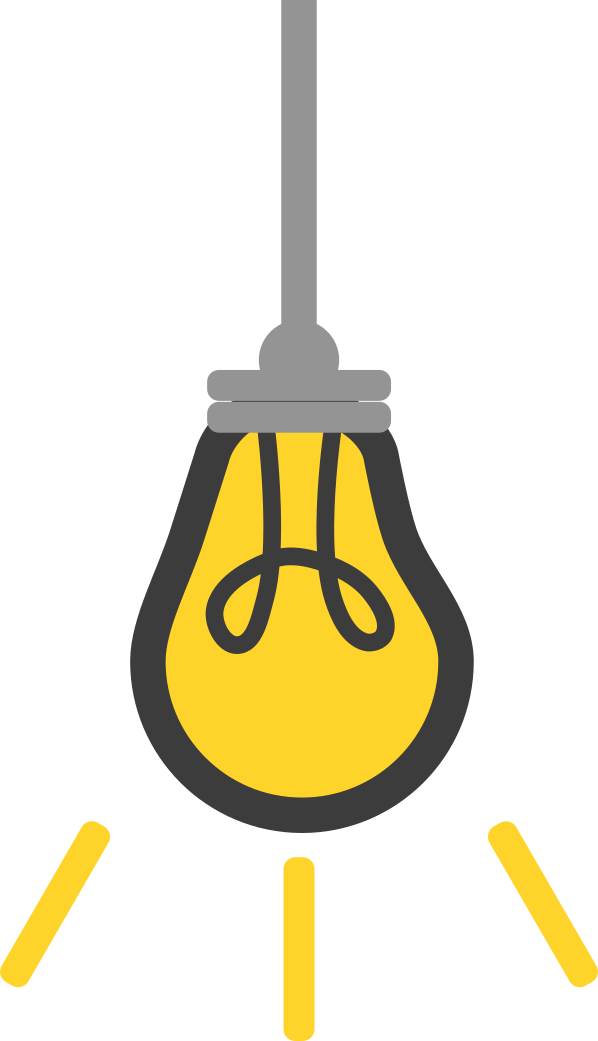
\includegraphics[angle=-30, origin=tr, width=1.5\textwidth]{lightbulb.png}
        \end{column}
    \end{columns}
\end{frame}

\section{Introduction}

\begin{frame}
    {What are hyperparameters?}
    \textbf{Hyperparameters} are values that are used by a ML model to control the learning process.

    Examples include:
    \begin{itemize}
        \item Structural parameters
              \begin{itemize}
                  \item Number of layers
                  \item Number of units in each layer
                  \item Number of filters, their kernel size, stride and padding
                  \item Type of activation function
                  \item \dots
              \end{itemize}
        \item Learning parameters
              \begin{itemize}
                  \item Type of optimizer
                  \item Learning rate $\alpha$
                  \item Schedule of learning rate
                  \item Loss function
                  \item Dropout rate
                  \item Weight regularization
                  \item \dots
              \end{itemize}
        \item \dots
    \end{itemize}

    \pause

    Other \textbf{parameters} such as weights and biases are learned by the network during training; these will be affected by the choice of hyperparameters.
\end{frame}

\begin{frame}
    {Problems with choosing hyperparameters}

    \begin{itemize}
        \item Deep network have an extremely large number of hyperparameters.
        \item The search space is extremely large but often the "good solution" only covers a small region of this space.
        \item We cannot try all possible combinations.
        \item No definitive strategy exists.
    \end{itemize}

    So... how do we choose hyperparameters?
\end{frame}

\section{Choosing hyperparameters}
\subsection{Manual methods}

\begin{frame}
    {What did others do?}
    We can look at the hyperparameters of published models that performed similar tasks and start from there.

    \textit{Pros}
    \begin{itemize}
        \item If others have used this successfully, there are good chances that might work.
        \item Computationally fast! :)
    \end{itemize}
    \pause
    \textit{Cons}
    \begin{itemize}
        \item It might be difficult to find a model doing exactly the same task.
    \end{itemize}
\end{frame}

\begin{frame}
    {Manual tweaking}
    \begin{itemize}
        \item Start with a reasonable choice of hyperparameters
        \item Modify one parameter at a time to improve model performance
    \end{itemize}
    \pause
    \textit{Pros}
    \begin{itemize}
        \item It generates high-quality results, when done by an expert.
        \item Humans can integrate knowledge from several sources and previous experience to make the best changes to hyperparameters.
    \end{itemize}
    \pause
    \textit{Cons}
    \begin{itemize}
        \item It is not obvious to find a good starting point.
        \item It is extremely time-consuming.
        \item There is no guarantee to find the optimal model.
        \item Difficult process to replicate.
    \end{itemize}
\end{frame}

\subsection{Automated methods}

\begin{frame}
    {Grid search}
    \textbf{Grid search} is the simplest method to use and is an exhaustive search over a defined parameter search space.

    \begin{columns}
        \begin{column}{.5\textwidth}
            \centering
            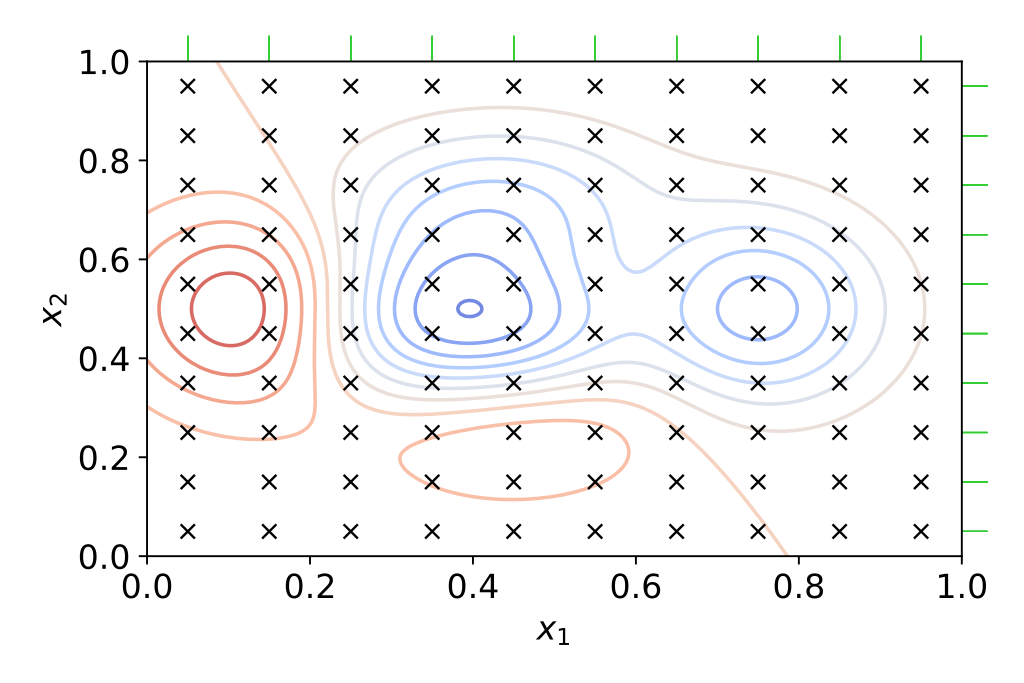
\includegraphics[width=\textwidth]{gridsearch.png}

            \footnotesize
            Grid search - In this example we tune hyperparameters $x_1$ and $x_2$ in the range $[0,1]$ - source Wikipedia
        \end{column}
        \begin{column}{.5\textwidth}
            \onslide<2->
            {
                \textit{Pros}
                \begin{itemize}
                    \item It is easy to implement.
                    \item Exhaustive search - guaranteed to find the optimal hyperparameters.
                    \item Reproducible.
                \end{itemize}
            }
            \onslide<3->{
                \textit{Cons}
                \begin{itemize}
                    \item It is computationally expensive -> early stop and parallelism help.
                    \item Need to choose a range.
                    \item It does not scale well; 5 hyperparameters with 10 values each, give $10^5$ combinations.
                    \item A lot of wasted computation time to sample low-accuracy combinations.
                \end{itemize}
            }
        \end{column}
    \end{columns}
\end{frame}

\begin{frame}
    {Grid search using Python}
    We will now see a simple implementation of grid search in Python.

    See the attached \texttt{GridSearch.ipynb} notebook.
\end{frame}

\begin{frame}
    {Random search}
    In \textbf{random search}, we randomly sample hyperparameters from the search space, rather than exploring a fixed grid.

    \begin{columns}
        \begin{column}{0.5\textwidth}
            \centering
            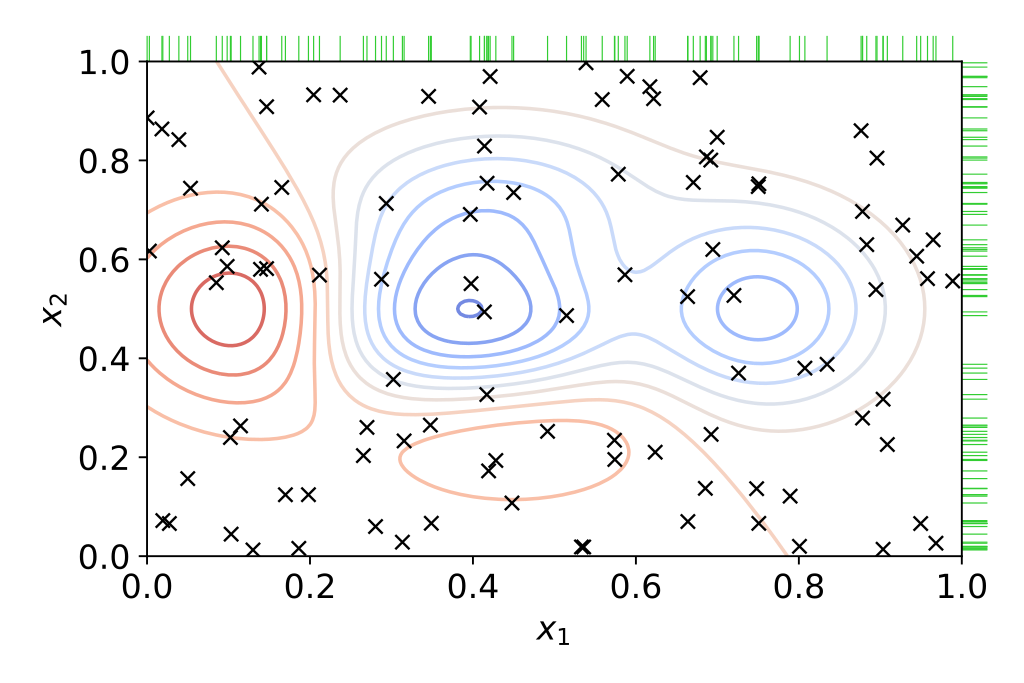
\includegraphics[width=\textwidth]{randomsearch.png}

            \footnotesize
            Random search - In this example we tune hyperparameters $x_1$ and $x_2$ in the range $[0,1]$. Random points are chosen in the grid space - source Wikipedia
        \end{column}
        \begin{column}{.5\textwidth}
            \onslide<2->
            {
                \textit{Pros}
                \begin{itemize}
                    \item Still easy to implement.
                    \item Helps when dealing with large search spaces.
                \end{itemize}
            }
            \onslide<3->{
                \textit{Cons}
                \begin{itemize}
                    \item Less reproducible.
                    \item Not guaranteed to hit the optimum.
                    \item Need to choose a range for the hyperparameters.
                \end{itemize}
            }
        \end{column}
    \end{columns}
\end{frame}

\begin{frame}
    {Bayesian optimization}
    \textbf{Bayesian} optimization, builds a probability model of the objective function; it uses this model to select the most promising set of hyperparameters. At each iteration, it updates its underlying model, and repeats the process.

    \begin{columns}
        \begin{column}{0.5\textwidth}
            \centering
            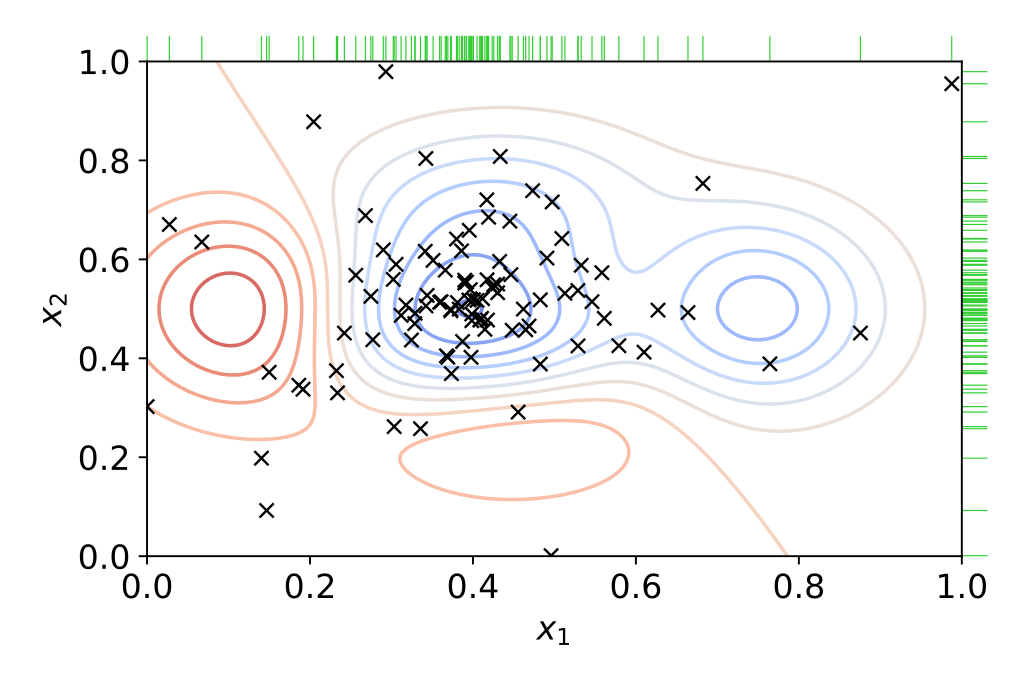
\includegraphics[width=\textwidth]{bayesian.png}

            \footnotesize
            Bayesian optimization - In this example we tune hyperparameters $x_1$ and $x_2$ in the range $[0,1]$. Bayesian optimization uses a statistical model to choose the next set of hyperparameters \textit{smartly} based on previous results - source Wikipedia
        \end{column}
        \begin{column}{.5\textwidth}
            \onslide<2->
            {
                \textit{Pros}
                \begin{itemize}
                    \item Efficient search of hyperparameter space.
                    \item Performs better than grid and random search.
                \end{itemize}
            }
            \onslide<3->{
                \textit{Cons}
                \begin{itemize}
                    \item Can be very computationally expensive when using a lot of hyperparameters.
                    \item Complex to implement.
                \end{itemize}
            }
        \end{column}
    \end{columns}
\end{frame}

\begin{frame}
    {Early-stopping based methods - Successive Halving}
    Early-stopping methods work by early stopping of evaluations on combinations of parameters that are not promising.

    \textbf{Successive Halving} algorithm

    \begin{itemize}[<+->]
        \item Choose a random set of $N$ hyperparameters configurations
        \item Set a maximum ``budget'' $B$ (e.g. number of epochs, time,\dots) to evaluate these configurations.
        \item Each configuration takes up $B/N$ of the budget.
        \item When the budget is exhausted, discard the worst-performing half of the configurations.
        \item Continues until only one configuration remains.
    \end{itemize}
    \pause
    \textbf{Problem}: do we consider a small $N$ with a large budget for each configuration, or a large $N$ with a small budget?
\end{frame}

\begin{frame}
    {Early-stopping based methods - Hyperband}
    \textbf{Hyperband} extends the Successive Halving algorithm by running multiple \textit{brackets} of hyperparameters.

    It performs a grid search on the number of configurations $N$ that we are going to choose.

    It can be 10-20x faster than Bayesian optimization.
\end{frame}

\section{KerasTuner}

\begin{frame}
    {KerasTuner}
    The \textbf{Keras Tuner} library (install via \texttt{pip install keras-tuner}) provides a simple way to tune hyperparameters in a Keras model.

    It implements the random search, Bayesian optimization and Hyperband strategies.

    In order to use Keras Tuner we need to have a function that generates and returns our Keras model. We will pass that function to the tuner class of our choice.
\end{frame}

\begin{frame}
    {KerasTuner example}
    \only<1>{
        \begin{codebox}
            \texttt{import keras\\
                import keras\_tuner as kt\\
                \\
                \# hp contains all the hyperparameters and is passed automatically by the tuner\\
                def build\_model(hp):\\
                $~~~~~~~~$model = keras.Sequential()\\
                $~~~~~~~~$\# Create an integer hyperparameter, going from 10 to 100\\
                $~~~~~~~~$\# We can also have hp.Float, hp.Choice, hp.Bool\\
                $~~~~~~~~$n\_filters = hp.Int('filters', min\_value=10, max\_value=100, step=10)\\
                $~~~~~~~~$model.add(keras.layers.Conv2D(n\_filters, (3, 3),\\
                $~~~~~~~~~~~~~~~~~~$input\_shape=(512, 512, 1)))\\
                $~~~~~~~~$$\dots$\\
                        $~~~~~~~~$model.compile($\dots$)\\
                        $~~~~~~~~$$\dots$\\
                    $~~~~~~~~$return model
            }
        \end{codebox}
    }
    \only<2>{
        \begin{codebox}
            \texttt{rs = kt.tuners.RandomSearch(build\_model,\\
                $~~~~~~~~$objective='val\_accuracy',\\
                $~~~~~~~~$max\_trials=10,\\
                $~~~~~~~~$directory="output\_dir")\\
                \\
                \# Instead of calling model.fit we call tuner.search\\
                rs.search(x\_train, y\_train,\\
                $~~~~~~~~$validation\_data=(x\_test, y\_test),\\
                $~~~~~~~~$epochs=10, batch\_size=32)\\
                \\
                best\_hyperparameter = rs.get\_best\_hyperparameters(1)[0]\\
                best\_model = rs.get\_best\_models(1)[0]\\
            }
        \end{codebox}
    }

    \pause
    We can now use a model with the best configuration for our task!
\end{frame}

\begin{frame}
    {Summary}
    \begin{itemize}
        \item Hyperparameters are values that control the learning process of a model.
        \item Manual methods are time-consuming, require expertise, and are not guaranteed to find the optimal model.
        \item Automated methods such as grid search, random search, Bayesian optimization, and early-stopping based methods can help.
        \item KerasTuner is a library that can help us tune hyperparameters in a Keras model.
    \end{itemize}
\end{frame}
\end{document}


